\section{Le moteur Unity}
\subsection{\textbf{Introduction}}

Unity est un moteur 2D/3D de développement temps réel, aujourd’hui largement répandu dans l’industrie du projet vidéo grâce à ses boîtes à outils particulièrement fournis permettant la création d’expériences interactives 2D, 3D.\\
En plus d'être un moteur de projet 2D/3D, Unity est également un environnement de développement intégré (IDE). Ainsi, il rassemble divers outils de développement que les développeurs utilisent souvent dans une interface graphique.\\
Par conséquent, la plateforme met à disposition un éditeur visuel qui offre la possibilité de simplement faire glisser et déposer différents éléments dans la scène. Qu'on peut ensuite modifier comme on le souhaite.\\
Le choix de ce moteur nous semble donc évident pour satisfaire nos besoins.

\subsection{\textbf{Fonctionnement interne et outils de développement}}

Unity \cite{unity} est un moteur de projet basé sur du C++ mais l'écriture du code est en C sharp, ce dernier permet de tester dans l'IDE sans aucun type d'exportation ou de construction. Lorsqu'on exécute notre code dans Unity, on utilise Mono version 3.5, qui a une compatibilité API à peu près équivalente à .NET Framework 3.5/CLR 2.0.\\
On peut utiliser MonoDevelop pour le débogage ou utiliser des plugins tiers pour Visual Studio, UnityVS.\\
MonoDevelop a un plugin qui ouvre une connexion au débogueur Unity et lui envoie des commandes après le débogage.\\

\subsection{\textbf{Un système de pipeline}}

Un système de pipeline \cite{pipeline} est un système qui permet de contrôler et d'adapter le rendu grâce à des scripts en C Sharp.\\

Sur Unity, il y a le choix entre trois systèmes de pipeline prédéfinis.\\

Le pipeline de rendu intégré standard est le pipeline de rendu par défaut de Unity. Il s'agit d'un pipeline de rendu à usage général qui dispose d'options de personnalisation limitées.\\

Le pipeline de rendu universel (URP) est un pipeline de rendu scriptable qui est rapide et facile à personnaliser et permet de créer des graphiques optimisés sur une large gamme de plateformes.\\

Le pipeline de rendu haute définition (HDRP) est un pipeline de rendu scriptable qui permet de créer des graphiques haute fidélité de pointe sur des plateformes haut de gamme.\\

On peut également créer notre propre pipeline de rendu à l'aide de l'API Scriptable Render Pipeline d'Unity.\\

Chacun des différents systèmes pipeline cible des types d'utilisations et des besoins matériels bien précis.\\

Dans notre cas on utilisera le pipeline de rendu intégré standard.

\subsection{\textbf{L'interaction avec la carte graphique}}

Le matériel graphique \cite{graphic} qui rend finalement la scène est contrôlé par un programme graphique spécial appelé Shaders. Les fonctionnalités matérielles sont progressivement améliorées au fil du temps et les fonctionnalités communes introduites à chaque étape sont appelées modèles de Shader. Le modèle de Shader progressif ajoute la prise en charge de programmes de shader plus longs, d'instructions de branchement plus puissantes et d'autres fonctionnalités, et ces améliorations permettent des améliorations parallèles des graphiques.\\

Unity permet d'obtenir des rendus graphiques en utilisant un modèle Shader inférieur ou au mieux aussi puissante que la carte graphique utilisée. \\

On peut également choisir le niveau d'émulation graphique, ceci est utile pendant le développement pour voir à quoi ressembleront les graphiques sur une machine plus ancienne.\\

Les performances de processeur au GPU (Graphics processing unit) diminuent jusqu’aux appels de dessin soumis à la carte graphique. Pour améliorer les performances, les appels de dessin doivent être stratégiquement réduits ou bien structurés afin d’obtenir des résultats optimaux. Étant donné que les appels de dessin eux-mêmes sont pleins de ressources, leur réduction réduira le travail global nécessaire. 

\subsection{\textbf{Lots d'appels de dessin}}

Le lot d'appels de dessin \cite{dessin} est une méthode d'optimisation des appels de dessin qui combine des maillages afin que Unity puisse les rendre en moins d'appels de dessin possible. \\

Unity fournit deux méthodes intégrées de traitement par lots des appels de dessin :\\

\textbf{- Traitement par lots statique} pour les GameObjects statiques, Unity les combine puis les assemble pour obtenir un rendu.\\

\textbf{- Mise en lot dynamique} pour les maillages suffisamment petits, cela transforme leurs sommets sur le CPU, regroupe les sommets similaires et les restitue en un seul appel de dessin.

\begin{center}
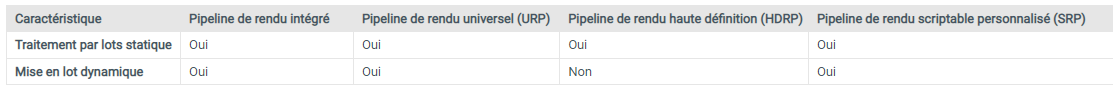
\includegraphics[height = 1.5cm]{images/pipeline.png}\\
\captionof{figure}{\small{Compatibilité du pipeline de rendu issue de la documentation officiel d'Unity}}
\end{center}

\subsection{\textbf{Version de logiciel utilisé}}

Les nouvelles versions \cite{version} disposent de fonctionnalités dont on aura pas besoin, on a donc choisi de travailler sur Unity version 2020.3.32f1 car cette version est stable et dispose de tout ce dont on a besoin afin de mener à bien notre projet.